\documentclass[a4paper]{article}
\usepackage[brazil]{babel}
\usepackage{fancyhdr}  % Pacote para editar cabeçalhos
\usepackage{graphicx}   % Pacote para inserir imagens
\usepackage{amsmath, amssymb}
\usepackage{geometry}
\usepackage{multicol}
\geometry{left=1cm,right=1cm,top=0.5cm,bottom=1cm}
\usepackage{enumitem}	
\usepackage{float} %for figure
\usepackage{titlesec}
\usepackage{setspace} %space between lines
\usepackage[many]{tcolorbox}  % for colores boxex (tikz and xcolor included)
\titleformat{\section}{\footnotesize\bfseries}{\thesection}{1em}{}
\usepackage{tikz}
\usepackage{keycommand}
\usetikzlibrary{arrows.meta,calc,decorations.pathreplacing}

%\singlespacing 
%\onehalfspacing %space between lines
%\doublespacing

% Remove a linha preta do cabeçalho
\renewcommand{\headrulewidth}{0pt}  

\pagestyle{fancy}  % Ativa o estilo de cabeçalho
\fancyhf{} % Limpa cabeçalhos e rodapés

% Adiciona as imagens no cabeçalho, ajustando a escala conforme necessário
\fancyhead[L]{\hspace{5cm}\raisebox{-3cm}{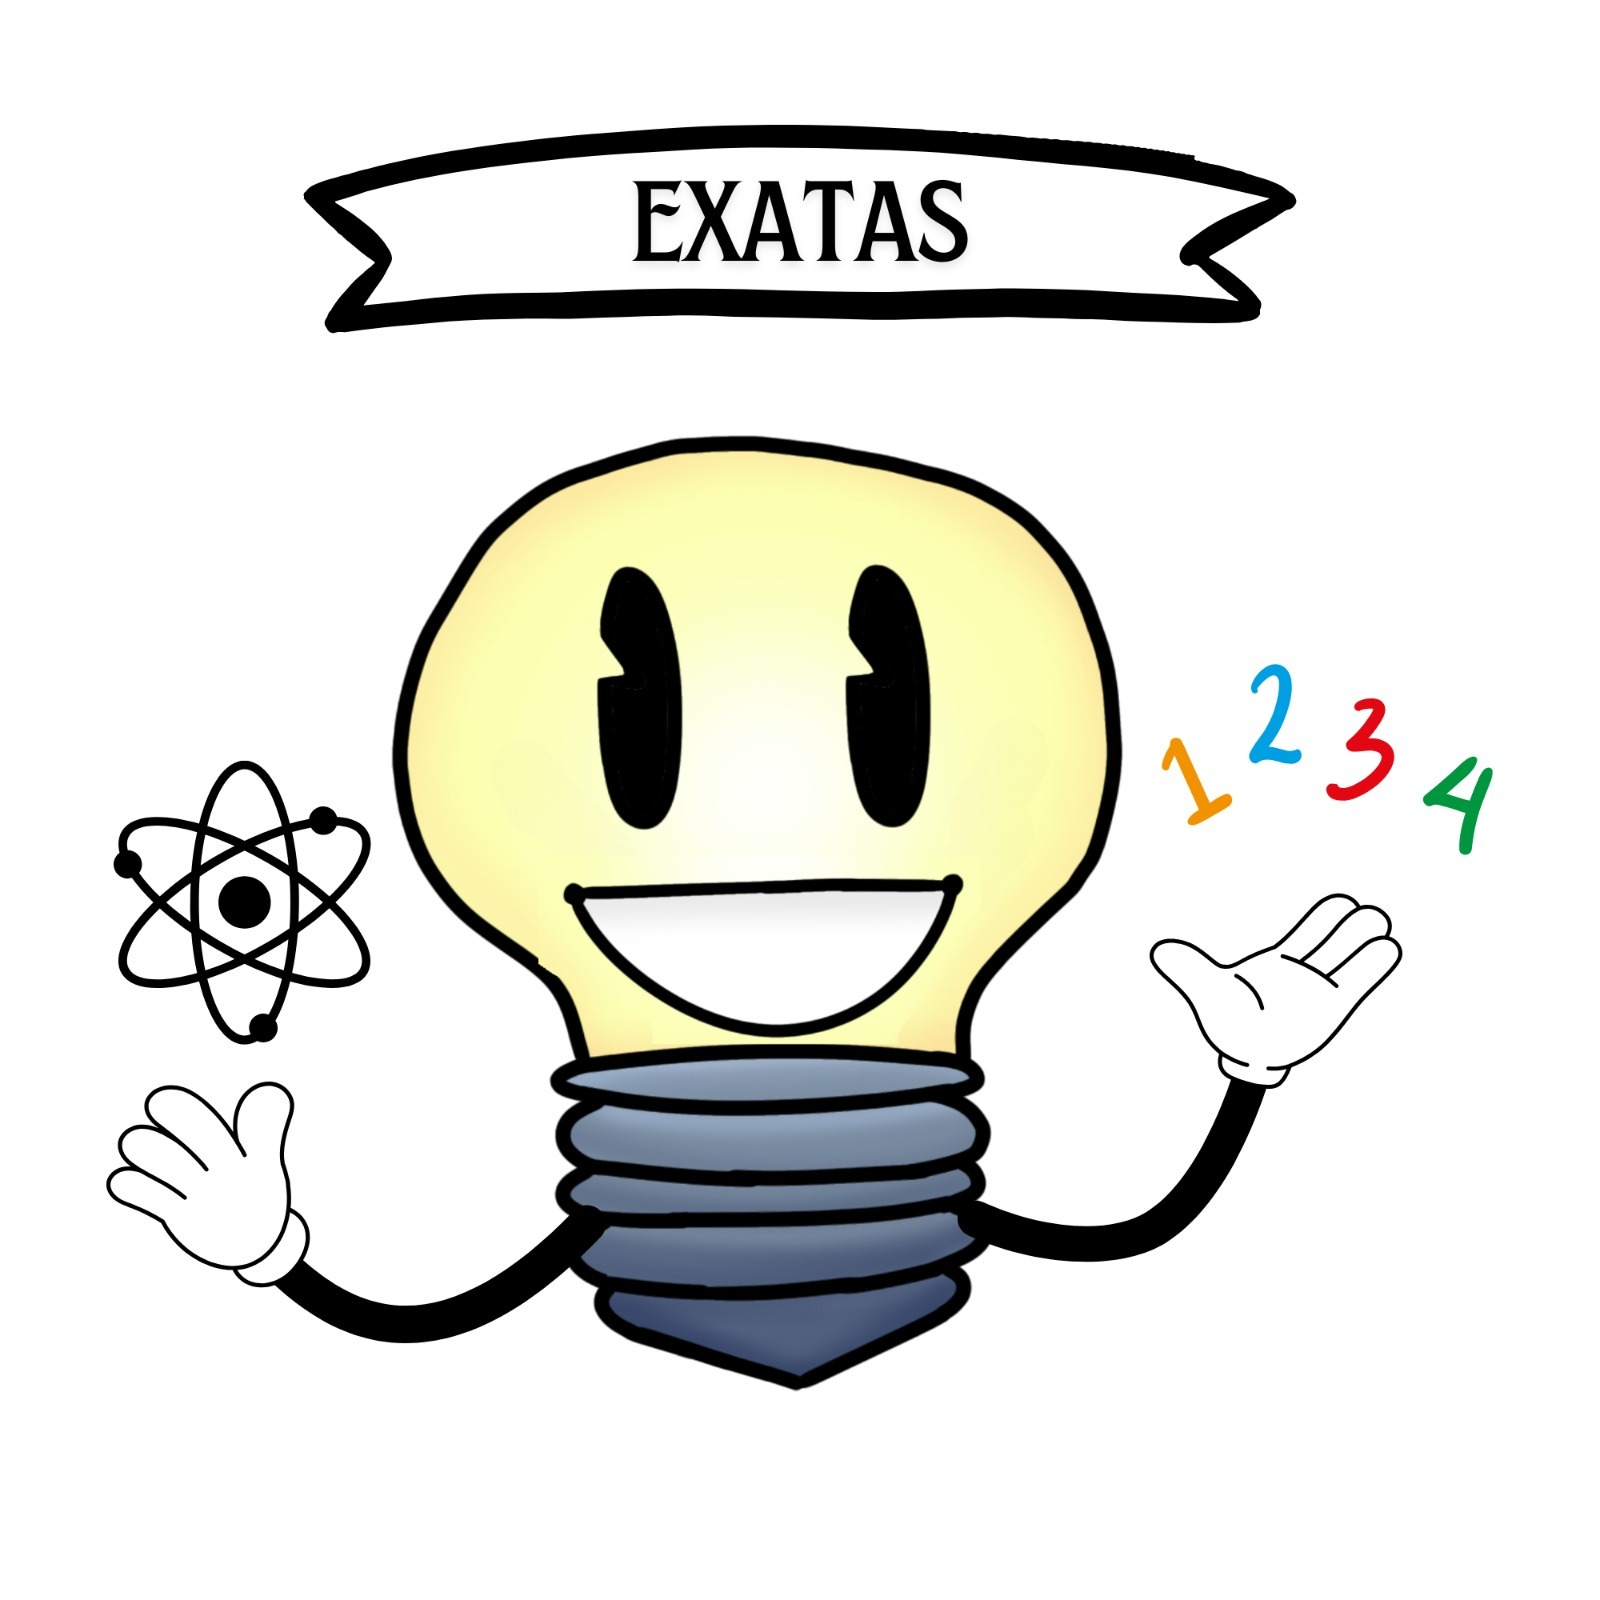
\includegraphics[width=2cm]{exata.jpg}}}  % Esquerda
\fancyhead[R]{\hspace{1cm}\raisebox{-2.8cm}{
\includegraphics[width=4cm]{pei.jpg}}} % Direita


%\newtcolorbox{boxA}{
%	fontupper = \bf,
%	boxrule = 1.5pt,
%	colframe = white  % frame color
	%rounded corners
	% arc = 5pt   % corners roundness	
%}



\begin{document}
	\fontsize{10}{15}\selectfont
	\vspace*{1mm}
	
	% ========= SEÇÃO: ATIVIDADE EXPRESSÕES ALGÉBRICAS ==========
	\section*{}	
	\begin{tcolorbox}[colback=gray!10, colframe=black, boxrule=0.5mm, arc=4pt, title=\textbf{Orientações}]
		A atividade deverá ser entregue até o dia \textbf{14/05}, com todas as resoluções feitas de forma completa e detalhada. 		
		Capriche nos cálculos e nas justificativas — isso será valorizado!
	\end{tcolorbox}
	
	\section*{PROBABILIDADE} 
				
	\begin{enumerate}
		\item Na Ilha de Matemática, há um santuário de aves que abriga somente araras azuis e papagaios verdes. Os biólogos observaram que há 150 araras azuis e 90 papagaios verdes vivendo no santuário. Eles também notaram que devido a migrações recentes, o número de araras azuis aumentou em 10\%, enquanto o número de papagaios verdes diminuiu em 5\%. Se um turista fotografar uma ave ao acaso no santuário, calcule a probabilidade de que a foto seja da:  \vspace*{-5mm}
		
		\begin{multicols}{3}[\setlength{\columnsep}{-1cm}]	
			\begin{enumerate}[]
				\item arara azul
				\item papagaio verde
				\item arara azul ou de um papagaio verde				
			\end{enumerate}
		\end{multicols}  \vspace*{-5mm}
		
		
		\item Miguel tem uma coleção de carrinhos composta por 8 carrinhos amarelos, 5 carrinhos brancos e 7 carrinhos verdes. Ele colocou todos esses carrinhos em sua mochila e foi até a casa de seu avô. Considerando que, ao chegar lá, Miguel retirou aleatoriamente um carrinho de sua mochila, qual a probabilidade de o carrinho retirado ser:  \vspace*{-5mm}
		
		\begin{multicols}{3}[\setlength{\columnsep}{-1cm}]	
			\begin{enumerate}[]
				\item amarelo
				\item branco
				\item verde				
			\end{enumerate}
		\end{multicols}  \vspace*{-5mm}
		
		\item
		Dois dados cúbicos, não viciados, com faces numeradas de 1 a 6, serão lançados simultaneamente. A probabilidade de que sejam sorteados dois números consecutivos, cuja soma seja um número primo, é de quanto?
		
		\item  Uma pesquisa revelou que 30\% dos alunos de uma escola praticam esportes e 20\% estudam música, mas 10\% praticam esportes e estudam música. Qual a probabilidade de um aluno, escolhido ao acaso, praticar esportes ou estudar música?
		
		\item Numa eleição para prefeito de uma certa
		cidade, concorreram somente os candidatos A e B. Em
		uma seção eleitoral, votaram 250 eleitores. Do número
		total de votos dessa seção, 42\% foram para o candidato A, 34\% foram para o candidato B, 18\% foram anulados e os restantes estavam em branco. Tirando-se, ao acaso, um voto dessa urna, a probabilidade de que seja um voto em branco é de quanto?
		
		\item A Coordenação de Matemática de uma
		escola promoveu uma gincana, na qual uma das tarefas
		era resolver o seguinte problema:
		“As faces de uma moeda são denominadas cara (K) e
		coroa (C). Se essa moeda for lançada 6 vezes, qual é a probabilidade de se obter 4 caras e 2 coroas?”
		Qual é a resposta correta para essa questão?
	\end{enumerate}			
\end{document}
